\documentclass[a4paper, 14pt]{extarticle}
\usepackage{float}
% Поля
%--------------------------------------
\usepackage{geometry}
\geometry{a4paper,tmargin=2cm,bmargin=2cm,lmargin=3cm,rmargin=1cm}
%--------------------------------------


%Russian-specific packages
%--------------------------------------
\usepackage[T2A]{fontenc}
\usepackage[utf8]{inputenc}
\usepackage[english, main=russian]{babel}
%--------------------------------------

\usepackage{textcomp}

% Красная строка
%--------------------------------------
\usepackage{indentfirst}
%--------------------------------------


%Graphics
%--------------------------------------
\usepackage{graphicx}
\graphicspath{ {./images/} }
\usepackage{wrapfig}
%--------------------------------------

% Полуторный интервал
%--------------------------------------
\linespread{1.3}
%--------------------------------------

%Выравнивание и переносы
%--------------------------------------
% Избавляемся от переполнений
\sloppy
% Запрещаем разрыв страницы после первой строки абзаца
\clubpenalty=10000
% Запрещаем разрыв страницы после последней строки абзаца
\widowpenalty=10000
%--------------------------------------

%Списки
\usepackage{enumitem}

%Подписи
\usepackage{caption}

%Гиперссылки
\usepackage{hyperref}

\hypersetup {
	unicode=true
}

%Рисунки
%--------------------------------------
\DeclareCaptionLabelSeparator*{emdash}{~--- }
\captionsetup[figure]{labelsep=emdash,font=onehalfspacing,position=bottom}
%--------------------------------------

\usepackage{tempora}

%Листинги
%--------------------------------------
\usepackage{listings}
\lstset{
  basicstyle=\ttfamily\footnotesize,
  %basicstyle=\footnotesize\AnkaCoder,        % the size of the fonts that are used for the code
  breakatwhitespace=false,        % sets if automatic breaks shoulbd only happen at whitespace
  breaklines=true,                 % sets automatic line breaking
  captionpos=t,                    % sets the caption-position to bottom
  inputencoding=utf8,
  frame=single,                    % adds a frame around the code
  keepspaces=true,                 % keeps spaces in text, useful for keeping indentation of code (possibly needs columns=flexible)
  keywordstyle=\bf,       % keyword style
  numbers=left,                    % where to put the line-numbers; possible values are (none, left, right)
  numbersep=5pt,                   % how far the line-numbers are from the code
  xleftmargin=25pt,
  xrightmargin=25pt,
  showspaces=false,                % show spaces everywhere adding particular underscores; it overrides 'showstringspaces'
  showstringspaces=false,          % underline spaces within strings only
  showtabs=false,                  % show tabs within strings adding particular underscores
  stepnumber=1,                    % the step between two line-numbers. If it's 1, each line will be numbered
  tabsize=2,                       % sets default tabsize to 8 spaces
  title=\lstname                   % show the filename of files included with \lstinputlisting; also try caption instead of title
}
%--------------------------------------

%%% Математические пакеты %%%
%--------------------------------------
\usepackage{amsthm,amsfonts,amsmath,amssymb,amscd}  % Математические дополнения от AMS
\usepackage{mathtools}                              % Добавляет окружение multlined
\usepackage[perpage]{footmisc}
%--------------------------------------

%--------------------------------------
%			НАЧАЛО ДОКУМЕНТА
%--------------------------------------

\begin{document}

%--------------------------------------
%			ТИТУЛЬНЫЙ ЛИСТ
%--------------------------------------
\begin{titlepage}
\thispagestyle{empty}
\newpage


%Шапка титульного листа
%--------------------------------------
\vspace*{-60pt}
\hspace{-65pt}
\begin{minipage}{0.3\textwidth}
\hspace*{-20pt}\centering

\includegraphics[width=\textwidth]{emblem}
\end{minipage}
\begin{minipage}{0.67\textwidth}\small \textbf{
\vspace*{-0.7ex}
\hspace*{-6pt}\centerline{Министерство науки и высшего образования Российской Федерации}
\vspace*{-0.7ex}
\centerline{Федеральное государственное бюджетное образовательное учреждение }
\vspace*{-0.7ex}
\centerline{высшего образования}
\vspace*{-0.7ex}
\centerline{<<Московский государственный технический университет}
\vspace*{-0.7ex}
\centerline{имени Н.Э. Баумана}
\vspace*{-0.7ex}
\centerline{(национальный исследовательский университет)>>}
\vspace*{-0.7ex}
\centerline{(МГТУ им. Н.Э. Баумана)}}
\end{minipage}
%--------------------------------------

%Полосы
%--------------------------------------
\vspace{-25pt}
\hspace{-35pt}\rule{\textwidth}{2.3pt}

\vspace*{-20.3pt}
\hspace{-35pt}\rule{\textwidth}{0.4pt}
%--------------------------------------

\vspace{1.5ex}
\hspace{-35pt} \noindent \small ФАКУЛЬТЕТ\hspace{80pt} <<Информатика и системы управления>>

\vspace*{-16pt}
\hspace{47pt}\rule{0.83\textwidth}{0.4pt}

\vspace{0.5ex}
\hspace{-35pt} \noindent \small КАФЕДРА\hspace{50pt} <<Теоретическая информатика и компьютерные технологии>>

\vspace*{-16pt}
\hspace{30pt}\rule{0.866\textwidth}{0.4pt}

\vspace{11em}

\begin{center}
\Large {\bf Лабораторная работа № 5.1} \\
\large {\bf по курсу <<Численные методы линейной алгебры>>} \\
\large <<Изучение сходимости метода Якоби>>
\end{center}\normalsize

\vspace{8em}


\begin{flushright}
  {Студент группы ИУ9-71Б Баев Д.А \hspace*{15pt}\\
  \vspace{2ex}
  Преподаватель Посевин Д. П.\hspace*{15pt}}
\end{flushright}

\bigskip

\vfill


\begin{center}
\textsl{Москва 2023}
\end{center}
\end{titlepage}
%--------------------------------------
%		КОНЕЦ ТИТУЛЬНОГО ЛИСТА
%--------------------------------------

\renewcommand{\ttdefault}{pcr}

\setlength{\tabcolsep}{3pt}
\newpage
\setcounter{page}{2}

\section{Задание}\label{Sect::task}
1. Реализовать метод Якоби.

2. Ввести критерий остановки итерационного процесса, используя равномерную норму.

3. Проверить решение путем сравнения с решением любым методом Гаусса.

4. Проверить выполнение условия диагонального преобладания.

5. Используя согласованную векторную и матричную нормы, проверить выполнение условия: ||P|| <= q < 1.

\newpage
\section{Исходный код}

Исходный код программы представлен в листингах~\ref{lst:code1}--~\ref{lst:code4}.

\begin{figure}[H]
\begin{lstlisting}[language={},caption={Реализация метода Якоби},label={lst:code1}]
def jacobi(A, b, delta=1e-6):
    n = len(A)
    x_prev = np.zeros(shape=(n, ))
    difference = np.array([1] * n)
    x_k = None
    while norm(difference) > delta:
        x_k = np.array([sum([b[i]] + [A[i][j] * x_prev[j] * -1 for j in range(n) if j != i]) / A[i][i] for i in range(n)])
        difference = x_k - x_prev
        x_prev = deepcopy(x_k)
    return x_k
\end{lstlisting}
\end{figure}

\begin{figure}[H]
\begin{lstlisting}[language={},caption={Вычисление норм вектора и матрицы},label={lst:code2}]
def norm(vector):
    return max(abs(vector))

def norm_matrix(matrix):
    return max([sum(abs(matrix[i][j]) for j in range(len(matrix[i])) if j != i) / abs(matrix[i][i]) for i in range(len(matrix))])
\end{lstlisting}
\end{figure}

\begin{figure}[H]
\begin{lstlisting}[language={},caption={Получение результатов и сравнение},label={lst:code3}]
n = 3
A = generate_matrix(n=n, diag=1)

if check_diag_dom(A):
    print('Matrix has diagonal dominance')
else:
    print('Matrix has not diagonal dominance')

print("||P|| = ", norm_matrix(A), "< 1")

x = np.random.uniform(-100, 100, size=(n, ))

b = mul_matrix_by_vector(matrix=A, vector=x)

gauss_answer = gauss(A, b)
jacobi_answer = jacobi(A, b)

print("Gauss: ", gauss_answer, " norm dif: ", norm(gauss_answer - x))
print("Jacobi", jacobi_answer, " norm dif: ", norm(jacobi_answer - x))
print("Real: ", x)
\end{lstlisting}
\end{figure}


\section{Результаты}

Результаты поиска решения СЛАУ методом Якоби со всеми необходимыми проверками и сравнениями приведены на рисунках~\ref{fig:img1}-~\ref{fig:img3}.


\begin{figure}[H]
\centering
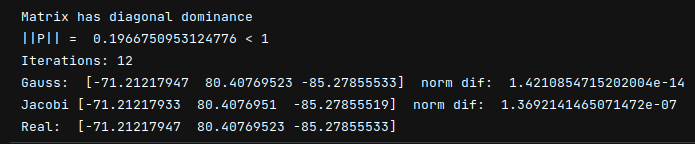
\includegraphics[width=0.8\textwidth]{images/res1.png}
\caption{Результат решения СЛАУ методом Якоби для матрицы 3x3}
\label{fig:img1}
\end{figure}


\begin{figure}[H]
\centering
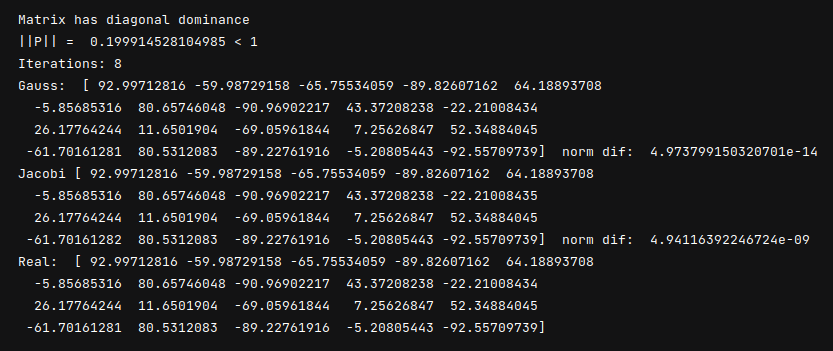
\includegraphics[width=0.8\textwidth]{images/res2.png}
\caption{Результат решения СЛАУ методом Якоби для матрицы 20x20}
\label{fig:img2}
\end{figure}


\begin{figure}[H]
\centering
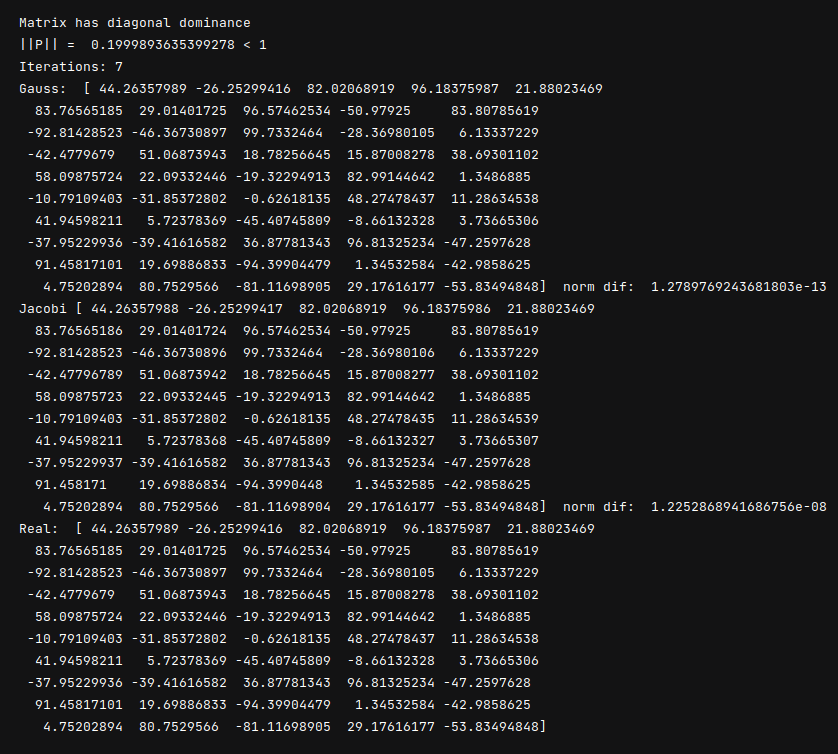
\includegraphics[width=0.8\textwidth]{images/res3.png}
\caption{Результат решения СЛАУ методом Якоби для матрицы 50x50}
\label{fig:img3}
\end{figure}


\section{Выводы}
В результате выполнения лабораторной работы был реализован и успешно протестирован метод Якоби решения системы линейных алгебраических уравнений. Также была реализована проверка достаточных условий сходимости этого метода.
\end{document}